\begin{figure}[!htbp]
\begin{center}

\begin{minipage}[t]{0.5\linewidth}

\begin{minipage}[t]{\linewidth}
\hspace*{\fill}%
\begin{minipage}[t]{0.05\linewidth}
\vspace{0pt} % for alignment
\rotatebox{90}{Messaging}%
\end{minipage}%
\hfill
\begin{minipage}[t]{0.45\linewidth}
\centering
\vspace{0pt} % for alignment
\adjincludegraphics[width=\textwidth, trim={{.0\width} {.0\width} {.5\width} {.5\width}}, clip]{img/knockout/intermessaging-sharing/wildtype/seed=1+title=directional_messaging_viz+treat=resource-wave__channelsense-yes__nlev-onebig+update=7172+_data_hathash_hash=f9e2a8ff33bf7745+_script_fullcat_hash=6b7e0389992dd616+_source_hash=53a2252-clean+ext=}%
\end{minipage}%
\hfill
\begin{minipage}[t]{0.45\linewidth}
\centering
\vspace{0pt} % for alignment
\adjincludegraphics[width=\textwidth, trim={{.0\width} {.0\width} {.5\width} {.5\width}}, clip]{img/knockout/intermessaging-sharing/knockout/seed=1+title=directional_messaging_viz+treat=resource-wave__channelsense-yes__nlev-onebig+update=7172+_data_hathash_hash=ffdeb1c77dd012e1+_script_fullcat_hash=6b7e0389992dd616+_source_hash=53a2252-clean+ext=}%
\end{minipage}%
\hspace*{\fill}

\hspace*{\fill}%
\begin{minipage}[t]{0.05\linewidth}
\vspace{0pt} % for alignment
\rotatebox{90}{Resource Sharing}%
\end{minipage}%
\hfill
\begin{minipage}[t]{0.45\linewidth}
\centering
\vspace{0pt} % for alignment
\adjincludegraphics[width=\textwidth, trim={{.0\width} {.0\width} {.5\width} {.5\width}}, clip]{img/knockout/intermessaging-sharing/wildtype/seed=1+title=directional_sharing_viz+treat=resource-wave__channelsense-yes__nlev-onebig+update=7172+_data_hathash_hash=f9e2a8ff33bf7745+_script_fullcat_hash=3a1e851383e0ffd4+_source_hash=53a2252-clean+ext=}%
\end{minipage}%
\hfill
\begin{minipage}[t]{0.45\linewidth}
\centering
\vspace{0pt} % for alignment
\adjincludegraphics[width=\textwidth, trim={{.0\width} {.0\width} {.5\width} {.5\width}}, clip]{img/knockout/intermessaging-sharing/knockout/seed=1+title=directional_sharing_viz+treat=resource-wave__channelsense-yes__nlev-onebig+update=7172+_data_hathash_hash=ffdeb1c77dd012e1+_script_fullcat_hash=3a1e851383e0ffd4+_source_hash=53a2252-clean+ext=}%
\end{minipage}%
\hspace*{\fill}

\hspace*{\fill}%
\begin{minipage}[t]{0.05\linewidth}
\vspace{0pt} % for alignment
\rotatebox{90}{Resource Stockpile}%
\end{minipage}%
\hfill
\begin{minipage}[t]{0.45\linewidth}
\centering
\vspace{0pt} % for alignment
\adjincludegraphics[width=\textwidth, trim={{.0\width} {.0\width} {.5\width} {.5\width}}, clip]{img/knockout/intermessaging-sharing/wildtype/seed=1+title=stockpile_viz+treat=resource-wave__channelsense-yes__nlev-onebig+update=7172+_data_hathash_hash=f9e2a8ff33bf7745+_script_fullcat_hash=4c8152cbf92e0da6+_source_hash=53a2252-clean+ext=}%
\end{minipage}%
\hfill
\begin{minipage}[t]{0.45\linewidth}
\centering
\vspace{0pt} % for alignment
\adjincludegraphics[width=\textwidth, trim={{.0\width} {.0\width} {.5\width} {.5\width}}, clip]{img/knockout/intermessaging-sharing/knockout/seed=1+title=stockpile_viz+treat=resource-wave__channelsense-yes__nlev-onebig+update=7172+_data_hathash_hash=ffdeb1c77dd012e1+_script_fullcat_hash=4c8152cbf92e0da6+_source_hash=53a2252-clean+ext=}%
\end{minipage}%
\hspace*{\fill}

\vspace{1.0ex}

\hspace*{\fill}%
\begin{minipage}[t]{0.05\linewidth}
\vspace{0pt} % for alignment
\end{minipage}%
\hfill
\begin{minipage}[t]{0.45\linewidth}
\centering
\vspace{0pt} % for alignment
Wild Type
\end{minipage}%
\hfill
\begin{minipage}[t]{0.45\linewidth}
\centering
\vspace{0pt} % for alignment
Messaging Knockout
\end{minipage}%
\hspace*{\fill}

\vspace{1.0ex}

% \begin{minipage}{\linewidth}
%   \caption{Phenotype visualizations}
%   \label{fig:intermessaging-sharing-phen}
% \end{minipage}

\end{minipage}%
% \begin{minipage}[t]{\linewidth}
%
% \hspace*{\fill}%
% \begin{minipage}[t]{\textwidth}
% \centering
% \vspace{0pt} % for alignment
% \begin{minipage}[b]{\textwidth}
% \includegraphics[width=\textwidth]{img/knockout/intermessaging-sharing/title=sharingdirection+_data_hathash_hash=59f6520a17fb3ad8+_script_fullcat_hash=97aad8dce5e50084+_source_hash=53a2252-clean+ext=}%
% \caption{Net sharing direction variance}
% \label{fig:intermessaging-sharing-direction}
% \end{minipage}
% \end{minipage}%
% \hfill
% \begin{minipage}[t]{\textwidth}
% \centering
% \vspace{0pt} % for alignment
% \begin{minipage}[b]{\textwidth}
% 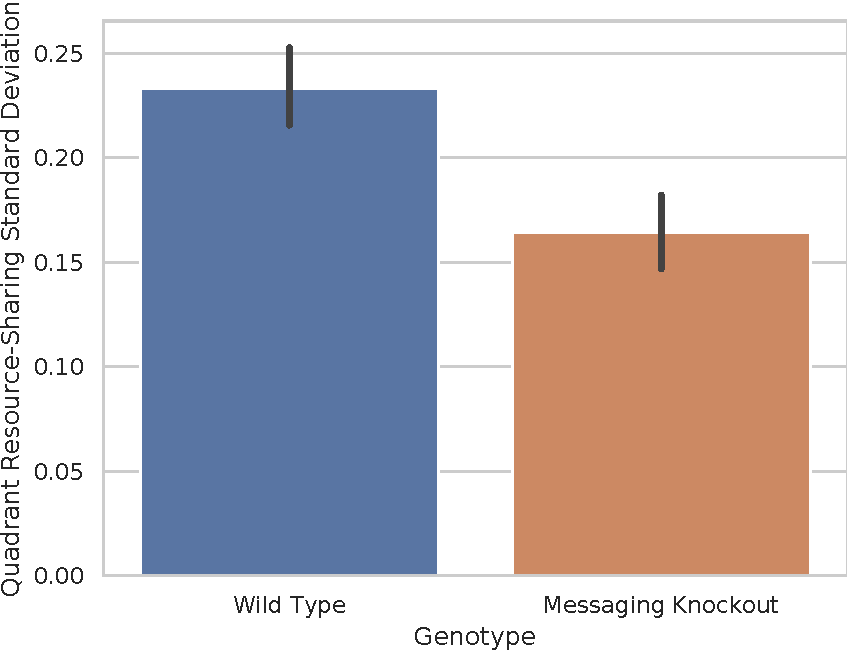
\includegraphics[width=\textwidth]{img/knockout/intermessaging-sharing/title=sharingquadrant+_data_hathash_hash=586f3c805332c323+_script_fullcat_hash=6e8aa37a96d9d7a9+_source_hash=53a2252-clean+ext=}%
% \caption{Net sharing localization variance}
% \label{fig:intermessaging-sharing-quadrant}
% \end{minipage}
% \end{minipage}%
% \hfill
% \begin{minipage}[t]{\textwidth}
% \centering
% \vspace{0pt} % for alignment
% \begin{minipage}[b]{\textwidth}
% \includegraphics[width=\textwidth]{img/knockout/intermessaging-sharing/title=fractionresevoir+_data_hathash_hash=7ce9af7e8fe0699b+_script_fullcat_hash=da31ee3af7ae0208+_source_hash=53a2252-clean+ext=}%
% \caption{Fraction of cells with enough resource to reproduce}
% \label{fig:intermessaging-sharing-resevoir}
% \end{minipage}
% \end{minipage}%
% \hspace*{\fill}
% \end{minipage}

\end{minipage}

\caption{
Visualization of phenotypic traits of a wild type strain evolved under the ``Flat-Wave'' treatment and corresponding intercell messaging knockout strain.
For these visualizations, group layouts are overlaid via borders between cells.
Black borders divide L0 hereditary groups.
In the messaging visualization, color coding represents the volume of incoming messages.
White represents no incoming messages and the magenta to blue gradient runs from one incoming message to the maximum observed incoming message traffic.
Unlike the wild type strain, as expected the messaging knockout strain exhibits no messaging activity.
In the resource sharing visualization, color coding represents the amount of incoming resource.
White represents no incoming resource and the magenta to blue gradient runs from the minimum to the maximum observed incoming incoming resource.
The wild type strain exhibits much more sparse resource sharing than the messaging knockout strain.
In the resource stockpile visualization, white represents zero-resource stockpiles, blue represents stockpiles with just under enough resource to reproduce, green represents stockpiles with enough resource to reproduce, and yellow represents more than enough resource to reproduce.
The wild type groups contain more cells with rich resource stockpiles (green and yellow) than the messaging knockout strain.
View an animation of the wild type strain at \url{https://hopth.ru/p}.
View the wild type strain in a live in-browser simulation at \url{https://hopth.ru/e}.
% minipages \ref{fig:intermessaging-sharing-direction}, \ref{fig:intermessaging-sharing-quadrant}, \ref{fig:intermessaging-sharing-resevoir} quantify knockout effects on various phenotypic traits.
% Error bars indicate 95\% confidence.
}
\label{fig:ko-intermessaging-sharing}
\end{center}
\end{figure}
